% Options for packages loaded elsewhere
\PassOptionsToPackage{unicode}{hyperref}
\PassOptionsToPackage{hyphens}{url}
%
\documentclass[
  12pt,
  ignorenonframetext,
]{beamer}
\usepackage{pgfpages}
\setbeamertemplate{caption}[numbered]
\setbeamertemplate{caption label separator}{: }
\setbeamercolor{caption name}{fg=normal text.fg}
\beamertemplatenavigationsymbolsempty
% Prevent slide breaks in the middle of a paragraph
\widowpenalties 1 10000
\raggedbottom
\setbeamertemplate{part page}{
  \centering
  \begin{beamercolorbox}[sep=16pt,center]{part title}
    \usebeamerfont{part title}\insertpart\par
  \end{beamercolorbox}
}
\setbeamertemplate{section page}{
  \centering
  \begin{beamercolorbox}[sep=12pt,center]{part title}
    \usebeamerfont{section title}\insertsection\par
  \end{beamercolorbox}
}
\setbeamertemplate{subsection page}{
  \centering
  \begin{beamercolorbox}[sep=8pt,center]{part title}
    \usebeamerfont{subsection title}\insertsubsection\par
  \end{beamercolorbox}
}
\AtBeginPart{
  \frame{\partpage}
}
\AtBeginSection{
  \ifbibliography
  \else
    \frame{\sectionpage}
  \fi
}
\AtBeginSubsection{
  \frame{\subsectionpage}
}
\usepackage{amsmath,amssymb}
\usepackage{iftex}
\ifPDFTeX
  \usepackage[T1]{fontenc}
  \usepackage[utf8]{inputenc}
  \usepackage{textcomp} % provide euro and other symbols
\else % if luatex or xetex
  \usepackage{unicode-math} % this also loads fontspec
  \defaultfontfeatures{Scale=MatchLowercase}
  \defaultfontfeatures[\rmfamily]{Ligatures=TeX,Scale=1}
\fi
\usepackage{lmodern}
\ifPDFTeX\else
  % xetex/luatex font selection
\fi
% Use upquote if available, for straight quotes in verbatim environments
\IfFileExists{upquote.sty}{\usepackage{upquote}}{}
\IfFileExists{microtype.sty}{% use microtype if available
  \usepackage[]{microtype}
  \UseMicrotypeSet[protrusion]{basicmath} % disable protrusion for tt fonts
}{}
\makeatletter
\@ifundefined{KOMAClassName}{% if non-KOMA class
  \IfFileExists{parskip.sty}{%
    \usepackage{parskip}
  }{% else
    \setlength{\parindent}{0pt}
    \setlength{\parskip}{6pt plus 2pt minus 1pt}}
}{% if KOMA class
  \KOMAoptions{parskip=half}}
\makeatother
\usepackage{xcolor}
\newif\ifbibliography
\usepackage{graphicx}
\makeatletter
\def\maxwidth{\ifdim\Gin@nat@width>\linewidth\linewidth\else\Gin@nat@width\fi}
\def\maxheight{\ifdim\Gin@nat@height>\textheight\textheight\else\Gin@nat@height\fi}
\makeatother
% Scale images if necessary, so that they will not overflow the page
% margins by default, and it is still possible to overwrite the defaults
% using explicit options in \includegraphics[width, height, ...]{}
\setkeys{Gin}{width=\maxwidth,height=\maxheight,keepaspectratio}
% Set default figure placement to htbp
\makeatletter
\def\fps@figure{htbp}
\makeatother
\setlength{\emergencystretch}{3em} % prevent overfull lines
\providecommand{\tightlist}{%
  \setlength{\itemsep}{0pt}\setlength{\parskip}{0pt}}
\setcounter{secnumdepth}{-\maxdimen} % remove section numbering
\usetheme{boxes}
%\usetheme{madrid} 
%\usetheme{metropolis} 
%\usetheme{Boadilla} 

%   \setbeameroption{show notes}  %the default is not to show notes

\usepackage{amsmath}
\setbeamertemplate{itemize items}[ball]
\setbeamertemplate{itemize subitem}[dash]
%\setbeamertemplate{frametitle}[default][center]
\setbeamertemplate{frametitle}[default][left]

%\setbeamertemplate{note page}[plain]
%\setbeamertemplate{note page}{\pagecolor{yellow!5}\insertnote}
\setbeamertemplate{note page}{\pagecolor{gray!15}\insertnote}

\usepackage[abs]{overpic}
\usepackage{wrapfig}
%\usepackage[table]{xcolor}
\usepackage{booktabs} %\toprule (and \midrule or \bottomrule) are defined in the booktabs package. 
%\usepackage{tabu}
\usepackage{longtable}
\usepackage{array}
\usepackage{multirow}
\usepackage{float}
\usepackage[most]{tcolorbox} %doesn't clash with the below
\usepackage{colortbl} 
\usepackage{pdflscape}
\usepackage{tabu}
\usepackage{threeparttable}
\usepackage{threeparttablex}
\usepackage[normalem]{ulem}
\usepackage{makecell}

% \usepackage{xcolor} %clashes with  \usepackage{colortbl}

\AtBeginNote{\hspace*{-5pt}\addtolength\leftmargini{-10pt}}
\AtEndNote{\addtolength\leftmargini{5pt}}

%\beamertemplatenavigationsymbolsempty
%\setbeamerfont{page number in head/foot}{size=\large}
\setbeamertemplate{footline}[frame number]                                       %page number

% defining a color
\definecolor{mossgreen}{rgb}{0.68, 0.87, 0.68}
\usepackage{mdframed}
\usepackage{framed}
\usepackage{scalerel,stackengine}

\usepackage{blindtext} %This package generates automatic text
\usepackage{epigraph}
\setlength\epigraphwidth{10cm}
\setlength\epigraphrule{0pt}
\makeatletter
\patchcmd{\epigraph}{\@epitext{#1}}{\itshape\@epitext{#1}}{}{}
\makeatother
\ifLuaTeX
  \usepackage{selnolig}  % disable illegal ligatures
\fi
\IfFileExists{bookmark.sty}{\usepackage{bookmark}}{\usepackage{hyperref}}
\IfFileExists{xurl.sty}{\usepackage{xurl}}{} % add URL line breaks if available
\urlstyle{same}
\hypersetup{
  pdftitle={Thinking Like an Economist},
  pdfauthor={Abel Embaye},
  hidelinks,
  pdfcreator={LaTeX via pandoc}}

\title{Thinking Like an Economist}
\author{Abel Embaye}
\date{September 08, 2025}
\institute{Department of Economics\\
\strut \\
UofA\\}

\begin{document}
\frame{\titlepage}

\begin{frame}{Chapter Outline}
\protect\hypertarget{chapter-outline}{}
10.1 Long-Run Economic Growth

10.2 Saving, Investment, and the Financial System

10.3 The Business Cycle
\end{frame}

\begin{frame}{10.1 Long-Run Economic Growth}
\protect\hypertarget{long-run-economic-growth}{}
\begin{itemize}
\item
  Long-run economic growth refers the average growth of the economy over
  several decades-- it is the process by which rising productivity
  increases the average standard of living.
\item
  This ignores the short-run swings in the economy inherent to the
  business cycle, the year to year fluctuation of the economy.
\item
  The average standard of living is measured by real GDP per capita.
\end{itemize}
\end{frame}

\begin{frame}{The Growth in Real GDP per Capita, 1900--2022}
\protect\hypertarget{the-growth-in-real-gdp-per-capita-19002022}{}
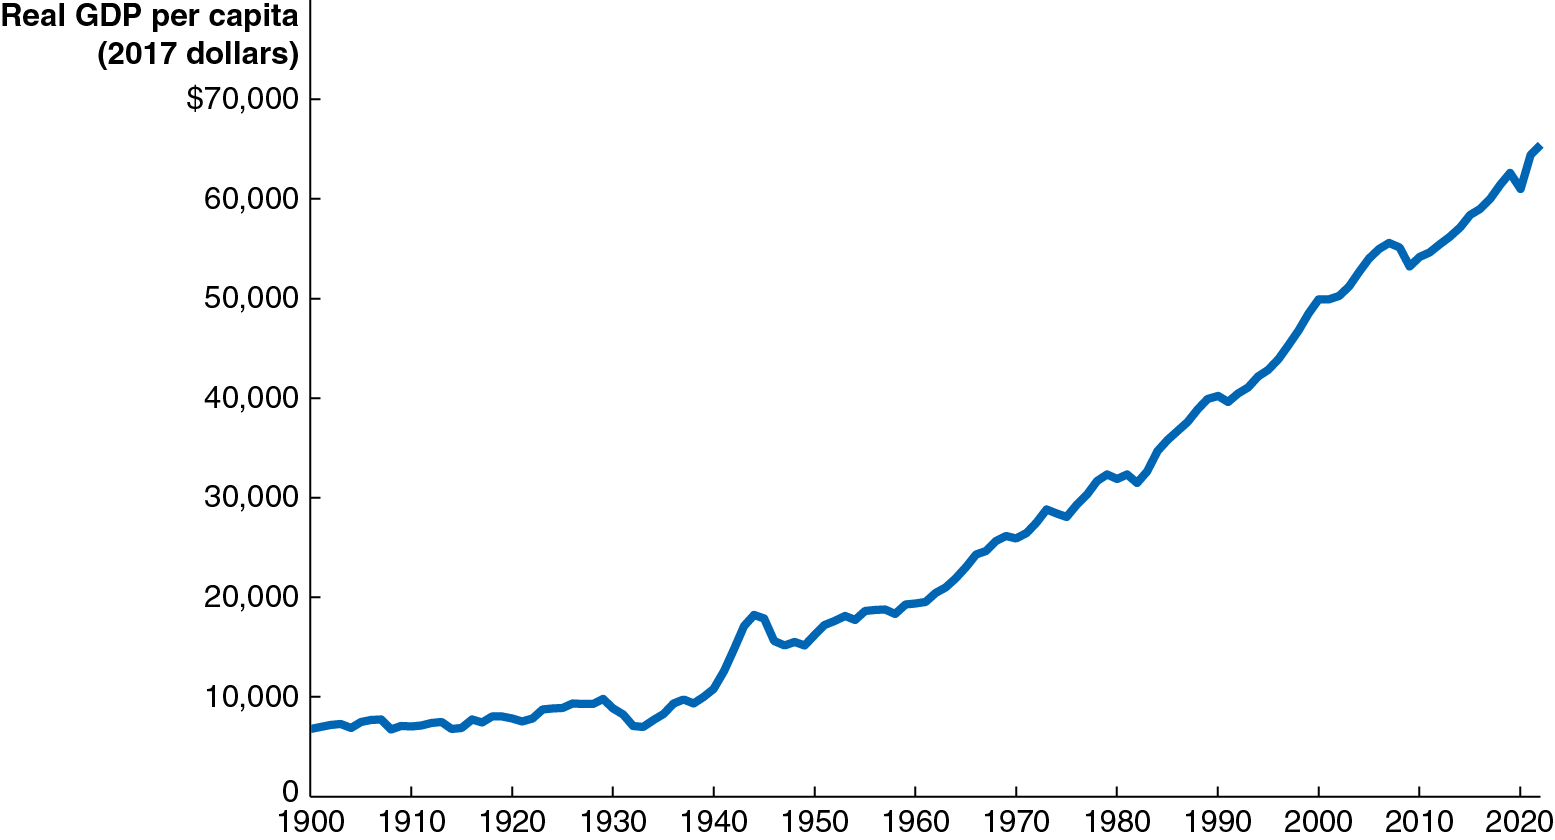
\includegraphics[width=\textwidth,height=0.99\textheight]{imgs3/img_slide06a.png}

Real GDP per capita has risen more than nine-fold since 1900-- the
average American can buy more than 9 times as many g\& s now as in 1900.
\end{frame}

\begin{frame}{Application: Economic Prosperity and Health}
\protect\hypertarget{application-economic-prosperity-and-health}{}
\begin{itemize}
\item
  Economic prosperity and health go hand in hand: richer nations can
  devote more resources to improving the health of their citizens, and
  healthier citizens are more productive.
\item
  Another good measure of our economic prosperity is the amount of time
  we can spend on leisure-- as our lifespan grows, we can spend more
  time on leisure; and also, as we grow more productive, we can devote
  less time to work, and hence more to leisure.
\end{itemize}
\end{frame}

\begin{frame}{Calculating Growth Rates}
\protect\hypertarget{calculating-growth-rates}{}
The growth rate of an economic variable like real GDP or real GDP per
capita is equal to the percentage change from one year to the next.

\begin{itemize}
\tightlist
\item
  In 2021, Real GDP was \$21.4 trillion + In 2022, Real GDP was \$21.8
  trillion
\end{itemize}
\end{frame}

\begin{frame}{Growth Rates over a Few Years}
\protect\hypertarget{growth-rates-over-a-few-years}{}
Over periods of a few years, we can average the growth rates to find the
approximate annual rate of growth. + In 2020, real GDP growth was -2.2\%
+ In 2021, real GDP growth was 5.8\% + In 2022, real GDP growth was
1.9\% + So, the average annual growth rate over this three-year period
was;
\end{frame}

\begin{frame}{Growth Rates over Longer Periods}
\protect\hypertarget{growth-rates-over-longer-periods}{}
Growth Rates over Longer Periods

For longer time periods, we wouldn't want to calculate each of the
annual growth rates and then take an average in order to find the
average annual growth rate; instead we would solve for the growth rate
g, where:

with t representing the number of time periods between the previous and
current periods. + A useful shortcut called the Rule of 70 can help us
determine how long it will take for an economic variable to double:

If the growth rate is 5 percent, the variable will double in
\end{frame}

\begin{frame}{What Determines the Rate of Long-Run Growth?}
\protect\hypertarget{what-determines-the-rate-of-long-run-growth}{}
What Determines the Rate of Long-Run Growth?

Increases in real GDP per capita rely on increases in labor
productivity: The quantity of goods and services that can be produced by
one worker or by one hour of work. + Why can the average American
consume more than nine times as many goods and services now than in
1900? + Because the average American produces more than nine times as
many goods and services in an hour now than in 1900.

So, most of the answer to ``what determines the rate of long-run
growth?'' is the same as the answer to ``what determines labor
productivity growth?''
\end{frame}

\begin{frame}{Factors Affecting Labor Productivity Growth (1 of 2)}
\protect\hypertarget{factors-affecting-labor-productivity-growth-1-of-2}{}
Factors Affecting Labor Productivity Growth (1 of 2)

Increases in capital per hour worked

Capital is physical assets and intellectual property that are used to
produce other goods and services. + The more capital a worker has
available to use (including human capital, the accumulated knowledge and
skills workers possess), the more productive he or she will be.

Technological change

Improvements in capital or methods to combine inputs into outputs (i.e.,
new technologies) allow workers to produce more in a given period of
time. + The role of entrepreneurs here is critical in pioneering new
ways to bring together the factors of production to produce better or
lower-cost products.
\end{frame}

\begin{frame}{Factors Affecting Labor Productivity Growth (2 of 2)}
\protect\hypertarget{factors-affecting-labor-productivity-growth-2-of-2}{}
Factors Affecting Labor Productivity Growth (2 of 2)

Property rights

A market system cannot function unless rights to private property are
secure. + Governments can aid growth by establishing independent court
systems to enforce contracts between private individuals.
\end{frame}

\begin{frame}{Apply the Concept: Can India Sustain Its Rapid Growth? (1
of 2)}
\protect\hypertarget{apply-the-concept-can-india-sustain-its-rapid-growth-1-of-2}{}
Apply the Concept: Can India Sustain Its Rapid Growth? (1 of 2)

To many people, the rapid economic rise of India was unexpected. +
Before its independence from England in 1947, growth rates in India were
very low, and India was desperately poor. + In 1991, the Indian
government decided to scale back central planning, reduce regulations,
and introduce market-based reforms, leading to the growth rate in
India's real GDP per capita doubling.

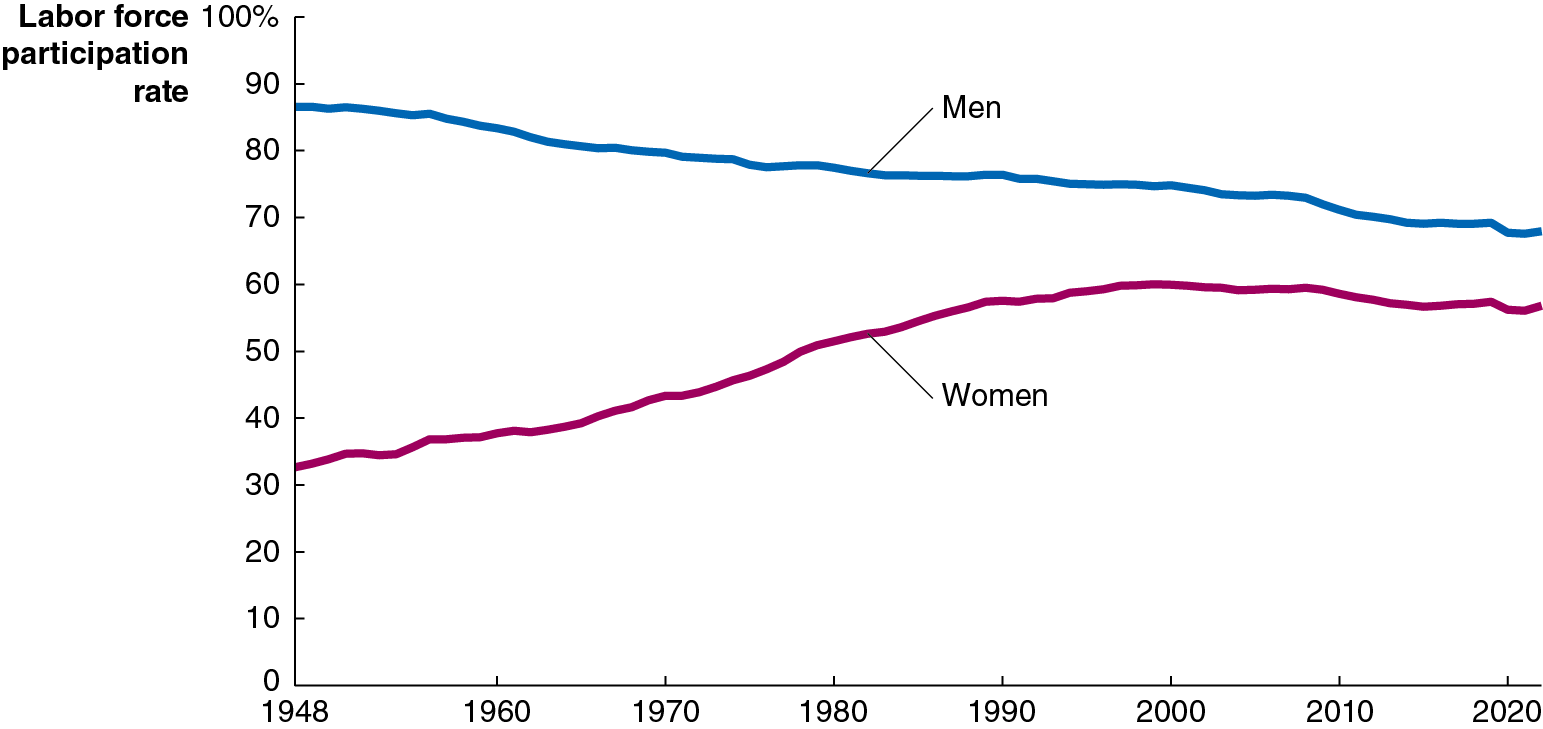
\includegraphics[width=\textwidth,height=0.99\textheight]{imgs3/img_slide15a.png}
\end{frame}

\begin{frame}{Apply the Concept: Can India Sustain Its Rapid Growth? (2
of 2)}
\protect\hypertarget{apply-the-concept-can-india-sustain-its-rapid-growth-2-of-2}{}
Apply the Concept: Can India Sustain Its Rapid Growth? (2 of 2)

Continued growth will require upgraded infrastructure, improved
educational and health services, and commitment to the rule of law and
market-based reforms. + Recent key policies in India include: +
Regulatory reforms to reduce corruption and improve the ability to
operate businesses. + Modernizing infrastructure, including roads,
railroads, and internet access.

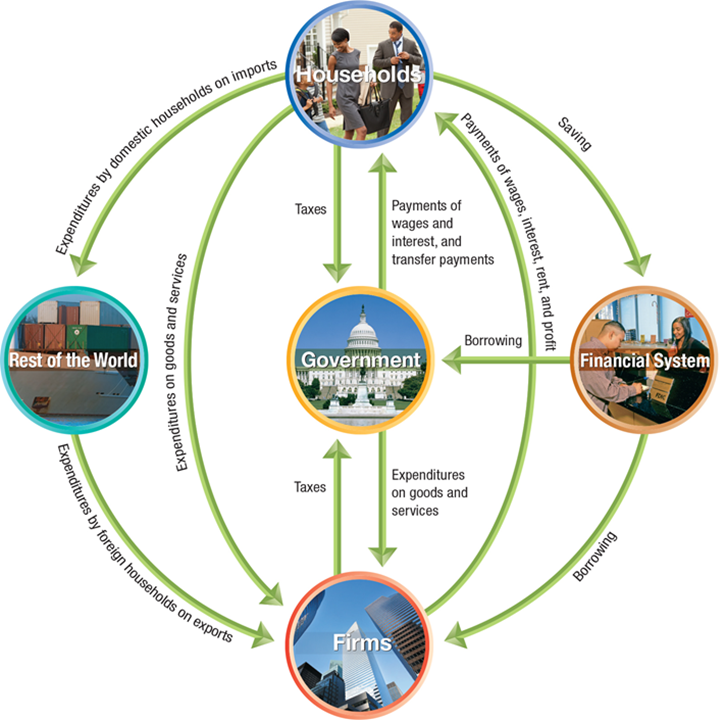
\includegraphics[width=\textwidth,height=0.99\textheight]{imgs3/img_slide16a.png}
\end{frame}

\begin{frame}{Potential GDP}
\protect\hypertarget{potential-gdp}{}
Potential GDP

Potential GDP is the level of real GDP attained when all firms are
operating at capacity. Capacity here refers to ``normal'' hours and a
``normal'' sized workforce. + Potential GDP rises when the labor force
expands, when a nation acquires more capital stock, or when new
technologies are created.

The growth in potential GDP in the United States has been relatively
steady at about 3.1 percent; that is, the potential to produce final
goods and services has been growing in the United States at about this
rate over time. + The recessions of 2007--2009 and 2020 resulted in a
wider than usual gap between potential and actual GDP, as the next slide
illustrates.
\end{frame}

\begin{frame}{Figure 10.2 Actual and Potential GDP}
\protect\hypertarget{figure-10.2-actual-and-potential-gdp}{}
Figure 10.2 Actual and Potential GDP

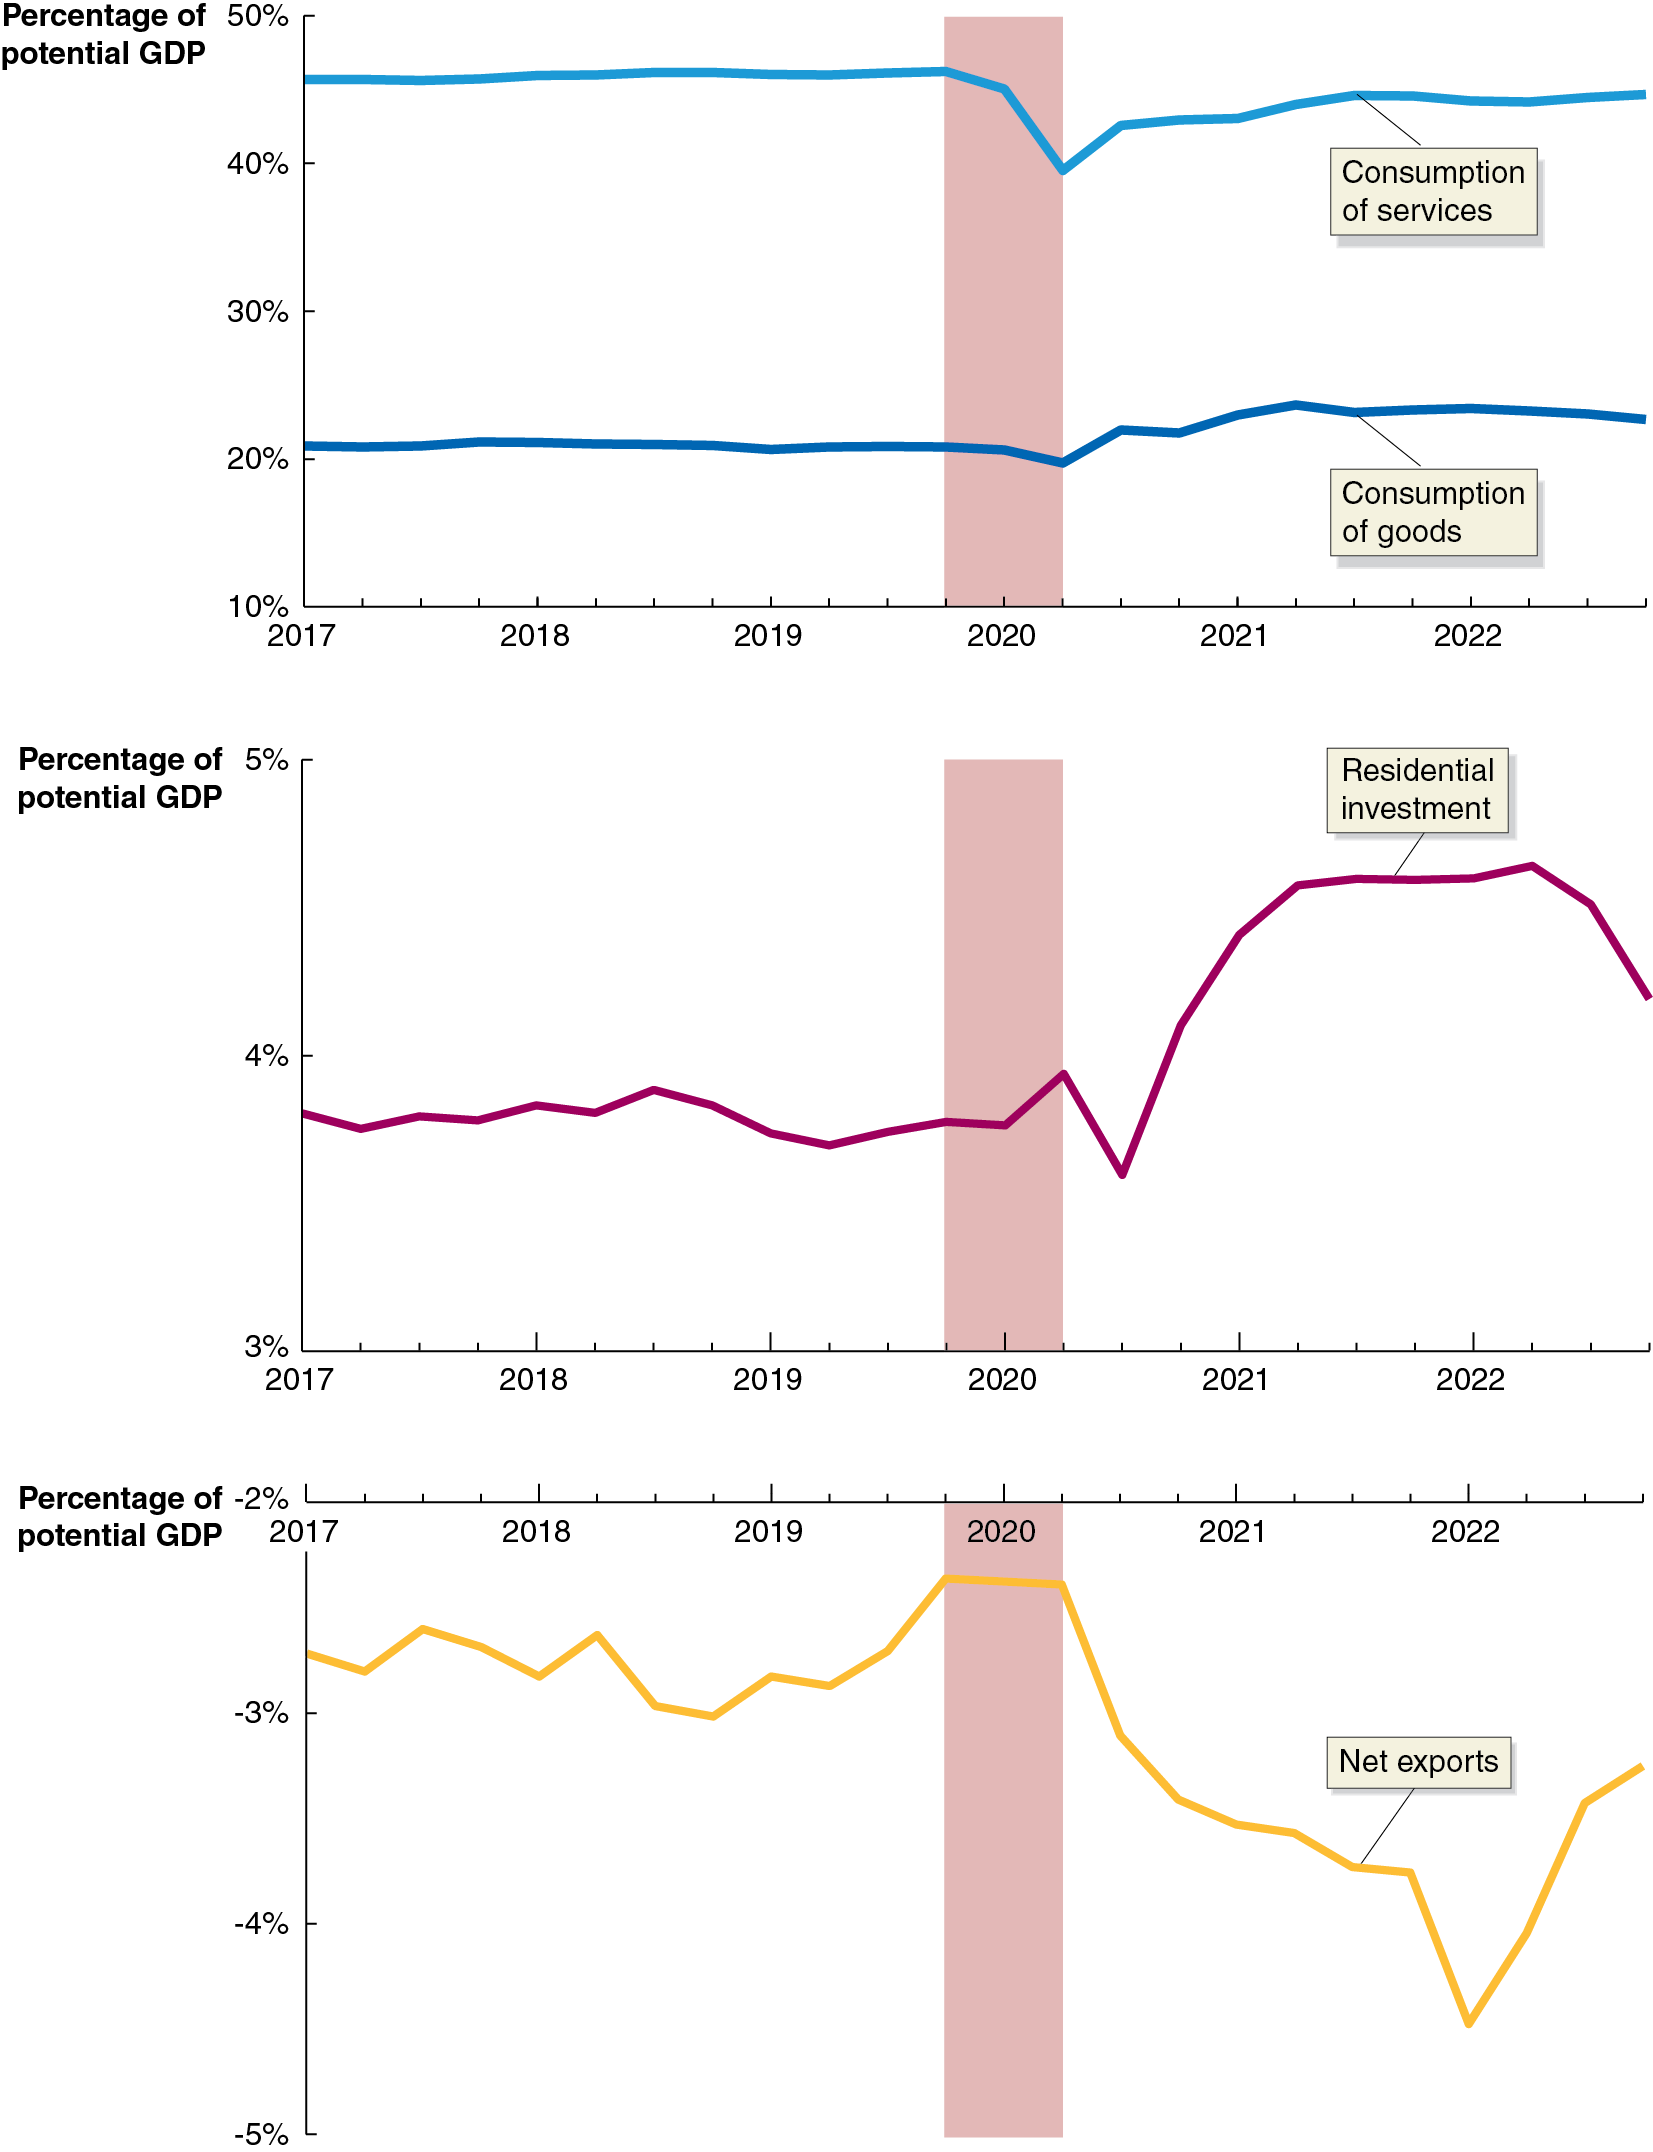
\includegraphics[width=\textwidth,height=0.99\textheight]{imgs3/img_slide18a.png}
\end{frame}

\begin{frame}{10.2 Saving, Investment, and the Financial System}
\protect\hypertarget{saving-investment-and-the-financial-system}{}
10.2 Saving, Investment, and the Financial System

Discuss the role of the financial system in facilitating long-run
economic growth.

Firms can finance some of their own expansion through retained earnings,
reinvesting profits back into the firm. + But often firms want to obtain
more funds for expansion than are available in this way.

Firms obtain these funds via the financial system: The system of
financial markets and financial intermediaries through which firms
acquire funds from households.
\end{frame}

\begin{frame}{Financial Markets and Financial Intermediaries}
\protect\hypertarget{financial-markets-and-financial-intermediaries}{}
Financial Markets and Financial Intermediaries

Financial markets are markets where financial securities, such as stocks
and bonds, are bought and sold. + Financial security: A document
(sometimes electronic) stating the terms under which funds pass from the
buyer of the security to the seller. + Stock: A financial security
representing partial ownership of a firm. + Bond: A financial security
promising to repay a fixed amount of funds. A bond is essentially a loan
from a household to a firm.

Financial intermediaries are firms, such as banks, mutual funds, pension
funds, and insurance companies, that borrow funds from savers and lend
them to borrowers.
\end{frame}

\begin{frame}{The Services the Financial System Provides}
\protect\hypertarget{the-services-the-financial-system-provides}{}
The Services the Financial System Provides

Risk sharing + By allowing investors to spread their money over many
different assets, investors can reduce their risk while maintaining a
high expected return on their investment.

Liquidity + The financial system allows savers to quickly convert their
investments into cash.

Information + The prices of financial securities represent the beliefs
of other investors and financial intermediaries about the future revenue
stream from holding those securities. + This aggregation of information
makes funds flow to the right firms.
\end{frame}

\begin{frame}{The Macroeconomics of Savings and Investment}
\protect\hypertarget{the-macroeconomics-of-savings-and-investment}{}
The Macroeconomics of Savings and Investment

We will now derive the result that the total value of saving in the
economy must equal the total value of investment. + Recall that we can
express the GDP of a nation (Y) as the sum of consumption (C),
investment (I), government purchases (G), and net exports (N X). That
is,

We will assume a closed economy, with no exports or imports; so

We can rearrange this to obtain an expression for investment:

That is, investment in a closed economy is equal to income minus
consumption and government purchases.
\end{frame}

\begin{frame}{Savings}
\protect\hypertarget{savings}{}
Savings

Savings is composed of private savings (by households,

and public savings (by the government,

is household income that is not spent; household income includes

payments for factors of production (Y) and transfer payments (T R);
households consume (C) and pay taxes (T). So,

The government ``saves'' whatever it brings in but does not spend (this
may be negative, known as dissaving):

So, total saving is:
\end{frame}

\begin{frame}{Savings Equals Investment}
\protect\hypertarget{savings-equals-investment}{}
Savings Equals Investment

The two previous slides led us to the same expressions for savings and
investment. So we conclude that savings must equal investment:

When

is zero, the government spends as much as it

brings in; this is known as a balanced budget. Negative and

positive values for

are known as budget deficits and

budget surpluses, respectively.

Since the federal government funds its current deficits with borrowing
(selling Treasury bonds), this takes away from the money available for
investment spending.
\end{frame}

\begin{frame}{The Market for Loanable Funds}
\protect\hypertarget{the-market-for-loanable-funds}{}
The Market for Loanable Funds

If savings must equal investments, how exactly does this occur? + The
financial system is composed of many different markets---the market for
stocks, for bonds, for certificates of deposits at banks, etc. + A
convenient way to model these is as a single market: the market for
loanable funds, a (conceptual) interaction of borrowers and lenders that
determines the market interest rate and the quantity of loanable funds
exchanged.

For now, we will assume that interactions are only between domestic
households and firms---there is no interaction with foreign lenders and
borrowers.
\end{frame}

\begin{frame}{Figure 10.3 The Market for Loanable Funds}
\protect\hypertarget{figure-10.3-the-market-for-loanable-funds}{}
Figure 10.3 The Market for Loanable Funds

Firms borrow loanable funds from households. They borrow more when
households demand a lower return on their money---a lower real interest
rate. + Households supply loanable funds to firms. They provide more
when firms offer them a greater reward for delaying consumption---a
higher real interest rate. + Governments, through their saving or
dissaving, affect the quantity of funds that ``pass through'' to firms.

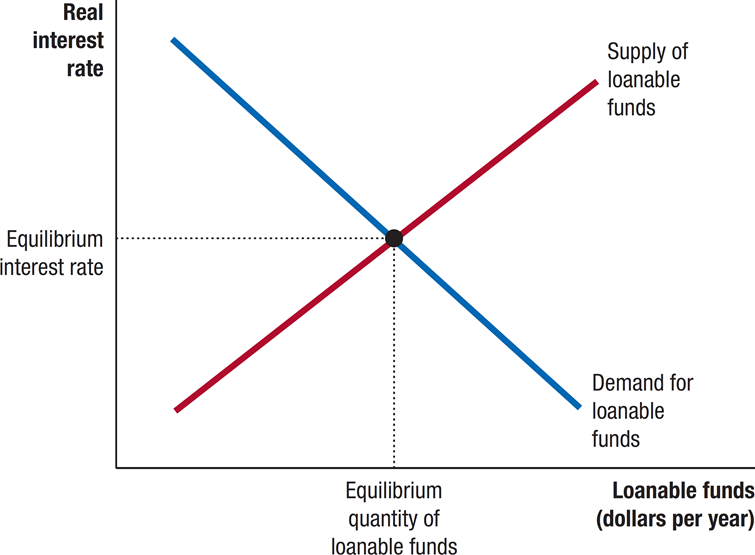
\includegraphics[width=\textwidth,height=0.99\textheight]{imgs3/img_slide26a.png}
\end{frame}

\begin{frame}{Apply the Concept: Ebenezer Scrooge: Accidental Promoter
of Economic Growth?}
\protect\hypertarget{apply-the-concept-ebenezer-scrooge-accidental-promoter-of-economic-growth}{}
Apply the Concept: Ebenezer Scrooge: Accidental Promoter of Economic
Growth?

In Charles Dickens's A Christmas Carol, Ebenezer Scrooge initially
spends little. In the book, this is portrayed negatively, but is this
really fair? + By declining to consume, Scrooge elects to save.
Society's resources can then be set toward investment, increasing
productive capacity and hence future consumption.

Eventually, Scrooge starts to spend his wealth. While this encourages
current production, society was probably better served---and achieved
stronger growth---when Scrooge chose to save instead.

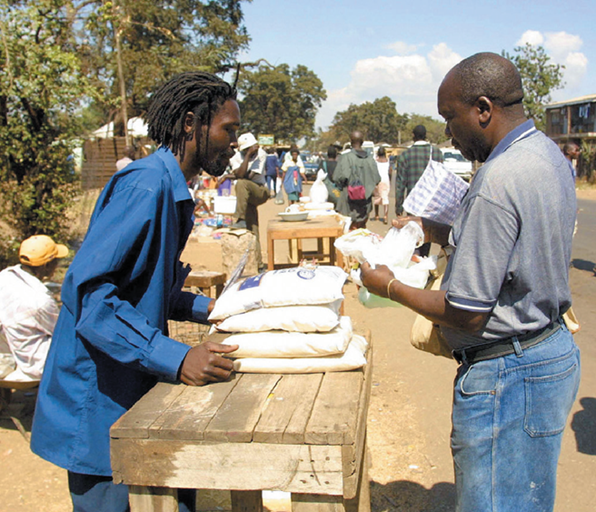
\includegraphics[width=\textwidth,height=0.99\textheight]{imgs3/img_slide27a.png}
\end{frame}

\begin{frame}{Figure 10.4 An Increase in the Demand for Loanable Funds}
\protect\hypertarget{figure-10.4-an-increase-in-the-demand-for-loanable-funds}{}
Figure 10.4 An Increase in the Demand for Loanable Funds

Suppose that technological change occurs so that investments become more
profitable for firms. + This will increase the demand for loanable
funds. + The real interest rate will rise, as will the quantity of funds
loaned.

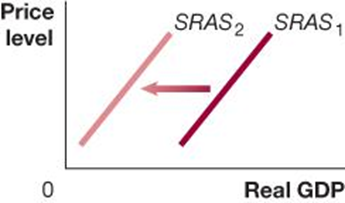
\includegraphics[width=\textwidth,height=0.99\textheight]{imgs3/img_slide28a.png}
\end{frame}

\begin{frame}{Figure 10.5 The Effect of a Budget Deficit on the Market
for Loanable Funds}
\protect\hypertarget{figure-10.5-the-effect-of-a-budget-deficit-on-the-market-for-loanable-funds}{}
Figure 10.5 The Effect of a Budget Deficit on the Market for Loanable
Funds

Suppose the government runs a budget deficit. + To fund the deficit, it
sells bonds to households, decreasing the supply of funds available to
firms. + This raises the equilibrium real interest rate and decreases
the funds loaned to firms. + This is crowding out: a decline in private
expenditure as a result of increases in government purchases.

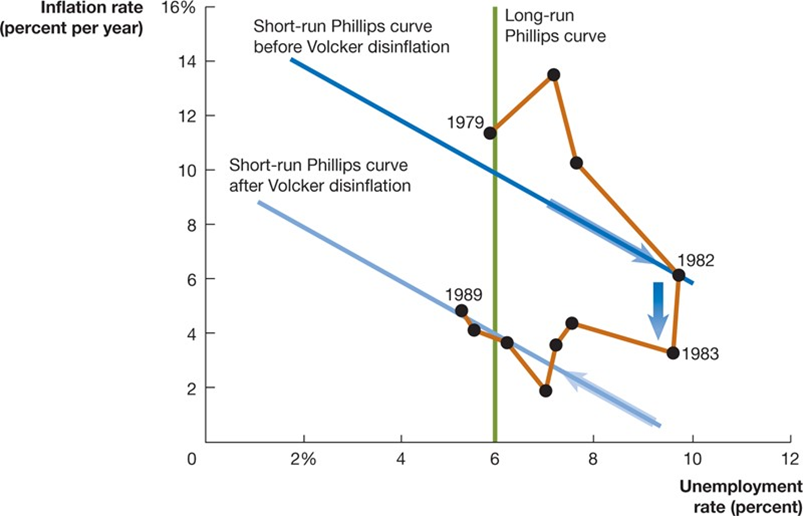
\includegraphics[width=\textwidth,height=0.99\textheight]{imgs3/img_slide29a.png}
\end{frame}

\begin{frame}{How Important Is Crowding Out?}
\protect\hypertarget{how-important-is-crowding-out}{}
How Important Is Crowding Out?

In practice, the effect of government budget deficits and surpluses on
the equilibrium interest rate is relatively small. + How small?
According to one study, increasing borrowing by 1 percent of GDP would
increase the real interest rate 0.003 points.

Why would the effect be so small? + Interest rates are influenced by
global markets, so even a few hundred billion dollars is a relatively
minor amount.
\end{frame}

\begin{frame}{Table 10.1 Summary of the Loanable Funds Model (1 of 2)}
\protect\hypertarget{table-10.1-summary-of-the-loanable-funds-model-1-of-2}{}
Table 10.1 Summary of the Loanable Funds Model (1 of 2)

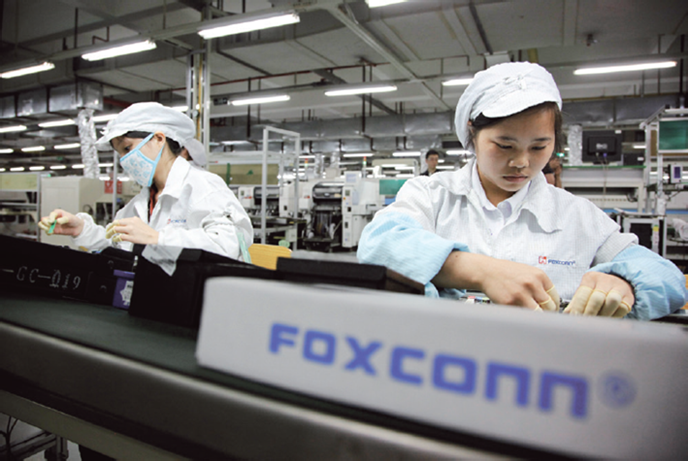
\includegraphics[width=\textwidth,height=0.99\textheight]{imgs3/img_slide31a.png}

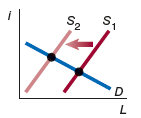
\includegraphics[width=\textwidth,height=0.99\textheight]{imgs3/img_slide31b.png}

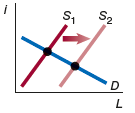
\includegraphics[width=\textwidth,height=0.99\textheight]{imgs3/img_slide31c.png}
\end{frame}

\begin{frame}{Table 10.1 Summary of the Loanable Funds Model (2 of 2)}
\protect\hypertarget{table-10.1-summary-of-the-loanable-funds-model-2-of-2}{}
Table 10.1 Summary of the Loanable Funds Model (2 of 2)

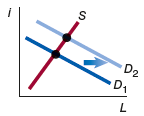
\includegraphics[width=\textwidth,height=0.99\textheight]{imgs3/img_slide32a.png}

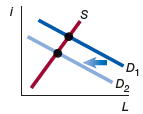
\includegraphics[width=\textwidth,height=0.99\textheight]{imgs3/img_slide32b.png}
\end{frame}

\begin{frame}{10.3 The Business Cycle}
\protect\hypertarget{the-business-cycle}{}
10.3 The Business Cycle

Explain what happens during the business cycle.

While real GDP per capita has risen about nine-fold since the start of
the twentieth century, it has not risen consistently every year. + Since
at least the early nineteenth century, the American economy has
experienced alternating periods of expanding and contracting economic
activity. + These alternating periods are called the business cycle.
\end{frame}

\begin{frame}{Figure 10.6 The Business Cycle (1 of 2)}
\protect\hypertarget{figure-10.6-the-business-cycle-1-of-2}{}
Figure 10.6 The Business Cycle (1 of 2)

The figure shows a typical idealized path for real GDP---rising,
falling, then rising again. + The phases of rising are known as
expansion; the periods of falling are recessions. + We refer to the
points at which the economy changes from one phase to the other as peaks
or troughs, respectively.


\includegraphics[width=\textwidth,height=0.99\textheight]{imgs3/img_slide34a.png}
\end{frame}

\begin{frame}{Figure 10.6 The Business Cycle (2 of 2)}
\protect\hypertarget{figure-10.6-the-business-cycle-2-of-2}{}
Figure 10.6 The Business Cycle (2 of 2)

This figure shows the movements in real GDP in the United States from
2006 to 2022. + The period of recession starting in late 2007 and ending
in mid-2009 was the longest and most severe since the Great Depression
of the 1930s, prompting some to refer to it as the Great Recession. + A
short but severe recession occurred during the first months of the
Covid-19 pandemic.

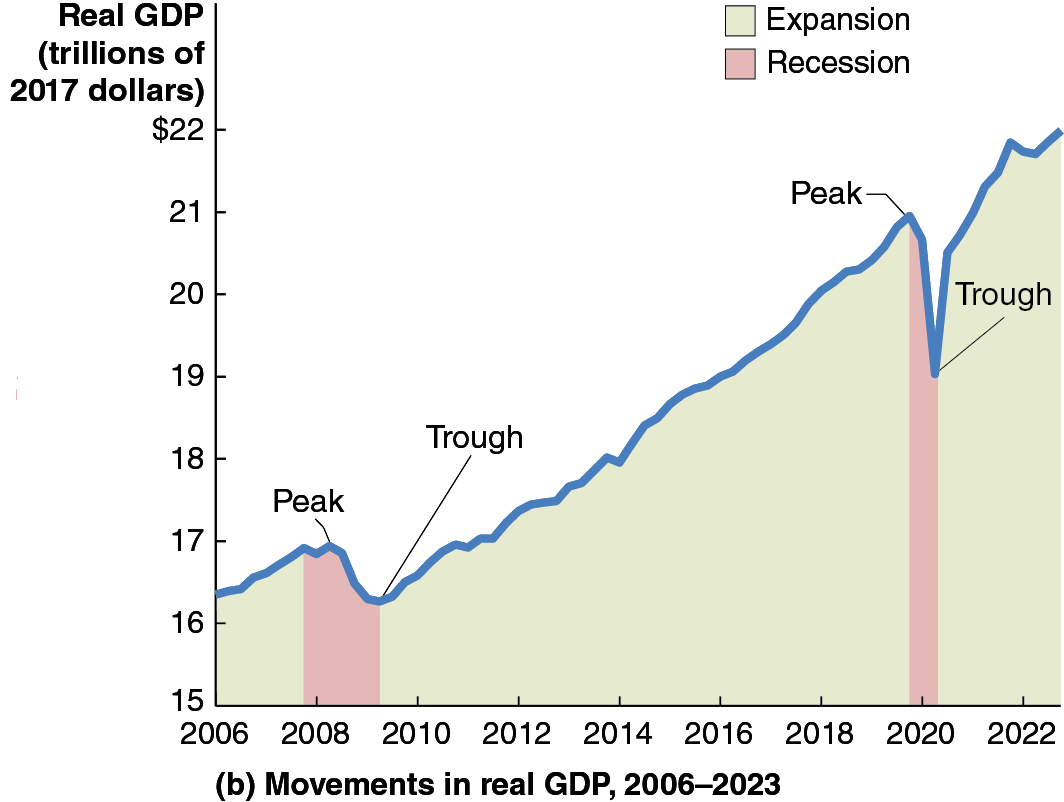
\includegraphics[width=\textwidth,height=0.99\textheight]{imgs3/img_slide35a.png}
\end{frame}

\begin{frame}{Table 10.2 The U.S. Business Cycle Since 1950 (1 of 2)}
\protect\hypertarget{table-10.2-the-u.s.-business-cycle-since-1950-1-of-2}{}
Table 10.2 The U.S. Business Cycle Since 1950 (1 of 2)

How do we know when the economy is in a recession? + The federal
government does not define when a recession starts or ends. + The
typical media definition of a recession is ``two consecutive quarters of
declining real GDP.''

Source: National Bureau of Economic Research.
\end{frame}

\begin{frame}{Table 10.2 The U.S. Business Cycle Since 1950 (2 of 2)}
\protect\hypertarget{table-10.2-the-u.s.-business-cycle-since-1950-2-of-2}{}
Table 10.2 The U.S. Business Cycle Since 1950 (2 of 2)

Most economists defer to the judgment of the National Bureau of Economic
Research (N B E R): + ``A recession is a significant decline in activity
spread across the economy, lasting more than a few months, visible in
industrial production, employment, real income, and wholesale-retail
trade.''

Source: National Bureau of Economic Research.
\end{frame}

\begin{frame}{What Happens during the Business Cycle?}
\protect\hypertarget{what-happens-during-the-business-cycle}{}
What Happens during the Business Cycle?

While each business cycle is different, most share these features: +
Near the end of an expansion, interest rates are rising, and the wages
of workers are rising faster than other prices.

Firm profits are falling.

As a recession begins, firms decrease their investment spending, and
households consume less.

Firms cut back on employment, leading to further declines in spending.

Eventually economic conditions improve; firms anticipate the future
expansion and begin investing again.

Households do too, and eventually employment recovers.
\end{frame}

\begin{frame}{The Effect of the Business Cycle on Inflation}
\protect\hypertarget{the-effect-of-the-business-cycle-on-inflation}{}
The Effect of the Business Cycle on Inflation

The inflation rate measures the change in the price level from one year
to the next. + During expansions, demand for products is high relative
to supply, resulting in prices increasing---high inflation. + During
recessions, demand for products is low relative to supply, resulting in
prices increasing more slowly or even decreasing---low inflation or
possibly deflation.

The graph on the next slide shows the movements in the (C P I) inflation
rate over the last two decades.
\end{frame}

\begin{frame}{Figure 10.7 The Effect of Recessions on the Inflation
Rate}
\protect\hypertarget{figure-10.7-the-effect-of-recessions-on-the-inflation-rate}{}
Figure 10.7 The Effect of Recessions on the Inflation Rate

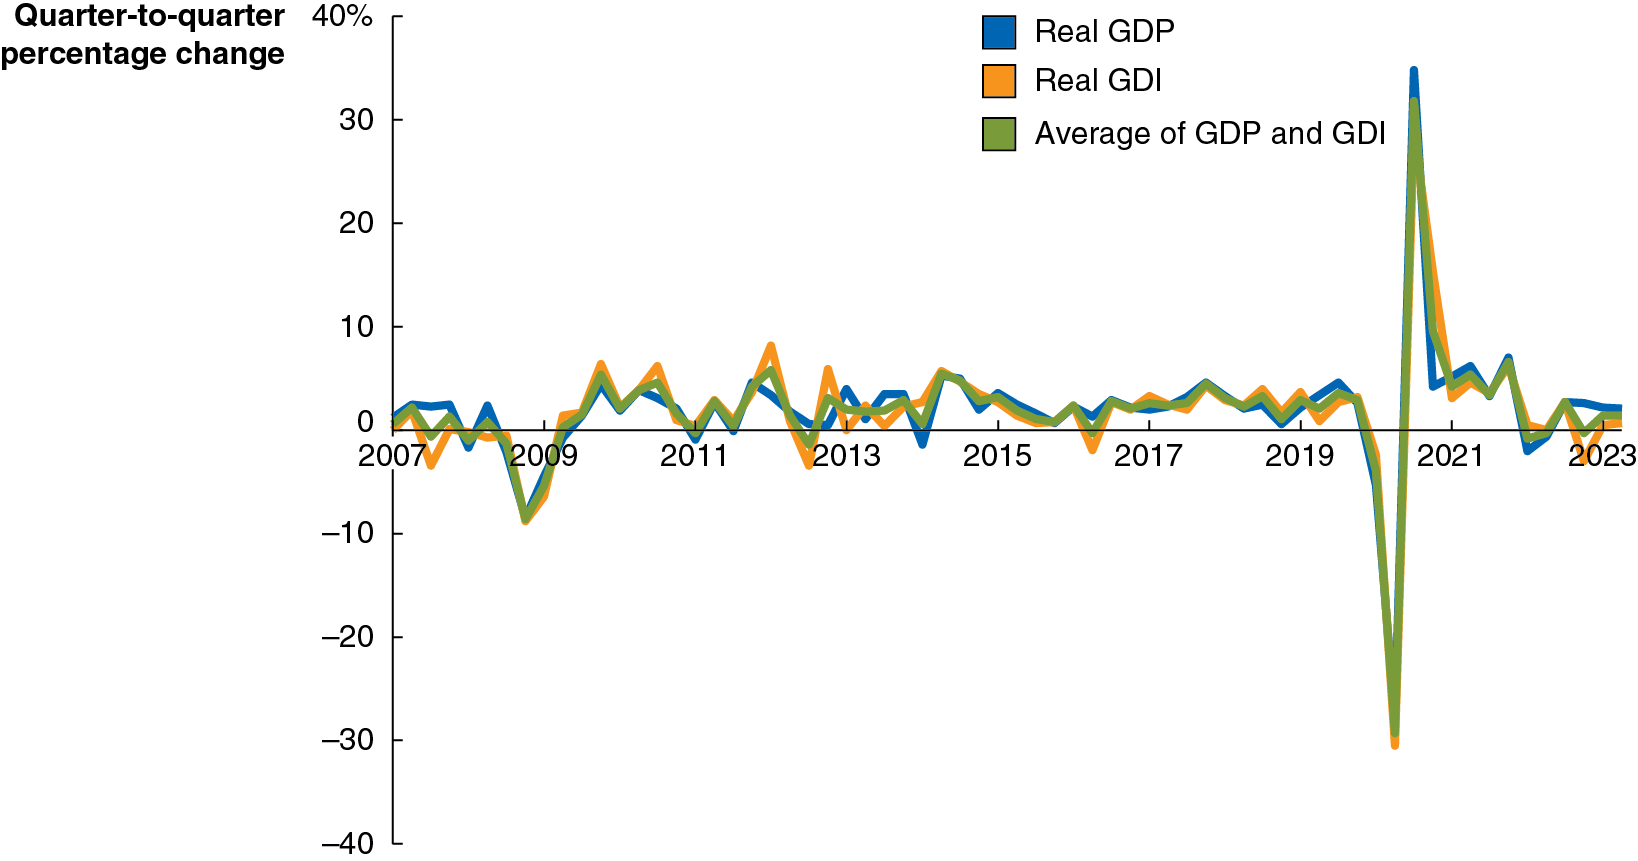
\includegraphics[width=\textwidth,height=0.99\textheight]{imgs3/img_slide40a.png}

Inflation tends to rise toward the end of an expansion and fall over the
course of each recession.
\end{frame}

\begin{frame}{Figure 10.8 How Recessions Affect the Unemployment Rate}
\protect\hypertarget{figure-10.8-how-recessions-affect-the-unemployment-rate}{}
Figure 10.8 How Recessions Affect the Unemployment Rate

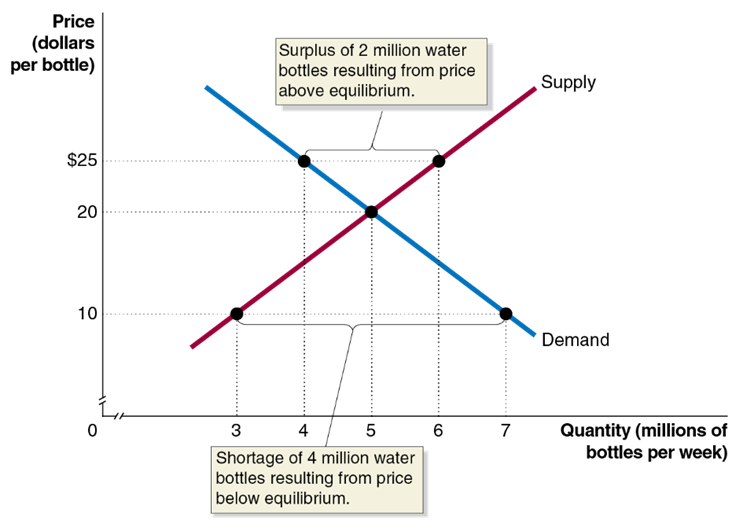
\includegraphics[width=\textwidth,height=0.99\textheight]{imgs3/img_slide41a.png}

As firms see their sales start to fall in a recession, they generally
reduce production and lay off workers. + Notice that unemployment often
continues to rise after the end of each recession.
\end{frame}

\begin{frame}{Figure 10.9 The Effect of the Great Recession and the 2020
Covid-19 Recession on Younger Workers}
\protect\hypertarget{figure-10.9-the-effect-of-the-great-recession-and-the-2020-covid-19-recession-on-younger-workers}{}
Figure 10.9 The Effect of the Great Recession and the 2020 Covid-19
Recession on Younger Workers

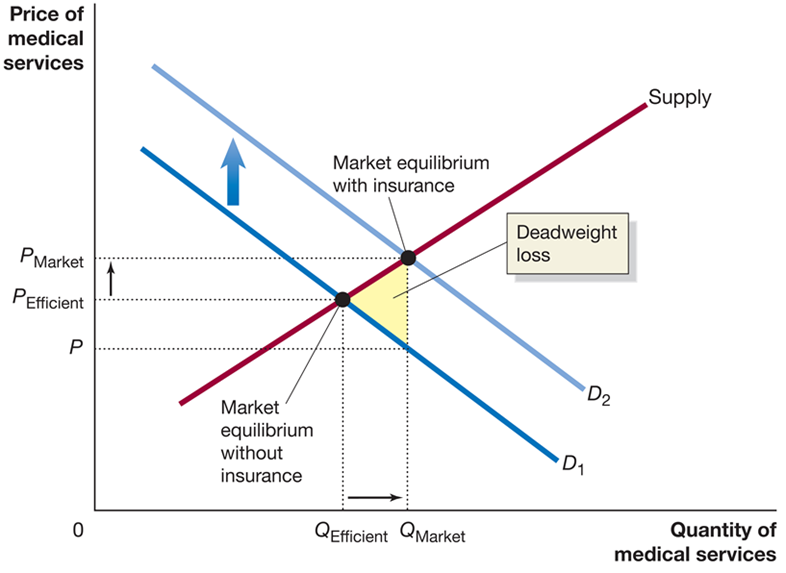
\includegraphics[width=\textwidth,height=0.99\textheight]{imgs3/img_slide42a.png}

Younger millennials were hit especially hard by the Great Recession.
Even now, those who were aged 20--24 in 2006 are less likely to be
employed than older workers. They saw similar impacts during the
Covid-19 recession of 2020. + Older millennials were also affected, but
less dramatically.
\end{frame}

\begin{frame}{Apply the Concept: Why Can't Economists Predict
Recessions?}
\protect\hypertarget{apply-the-concept-why-cant-economists-predict-recessions}{}
Apply the Concept: Why Can't Economists Predict Recessions?

Queen Elizabeth

visited the

London School of Economics during the 2008 financial crisis, and asked
``Why did nobody notice it?'' + Why can't economists predict recessions?
+ Business cycles are not uniform. + Leading economic indicators are not
reliable. + Events that trigger a recession are hard to predict.

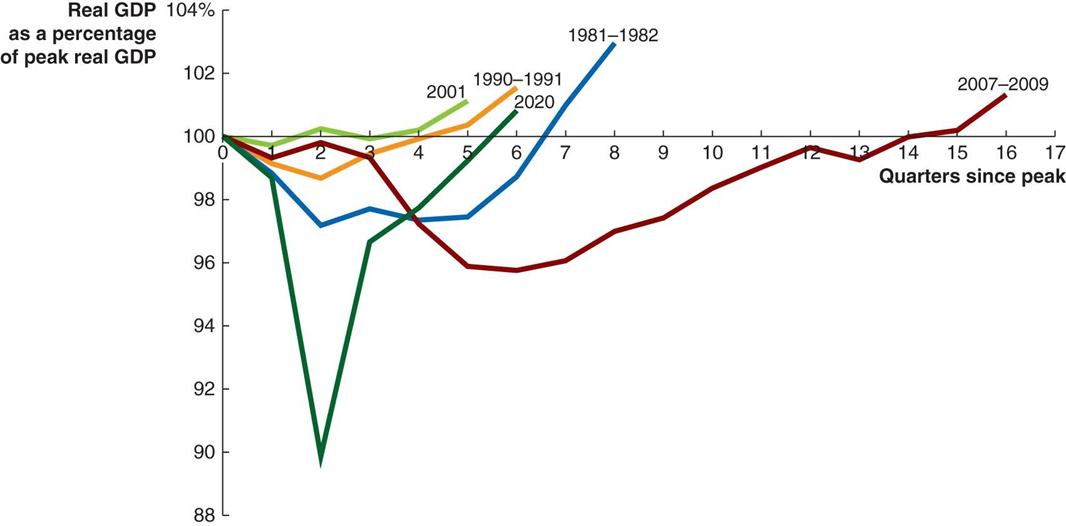
\includegraphics[width=\textwidth,height=0.99\textheight]{imgs3/img_slide43a.png}
\end{frame}

\begin{frame}{Figure 10.10 Fluctuations in Real GDP, 1900--2022}
\protect\hypertarget{figure-10.10-fluctuations-in-real-gdp-19002022}{}
Figure 10.10 Fluctuations in Real GDP, 1900--2022

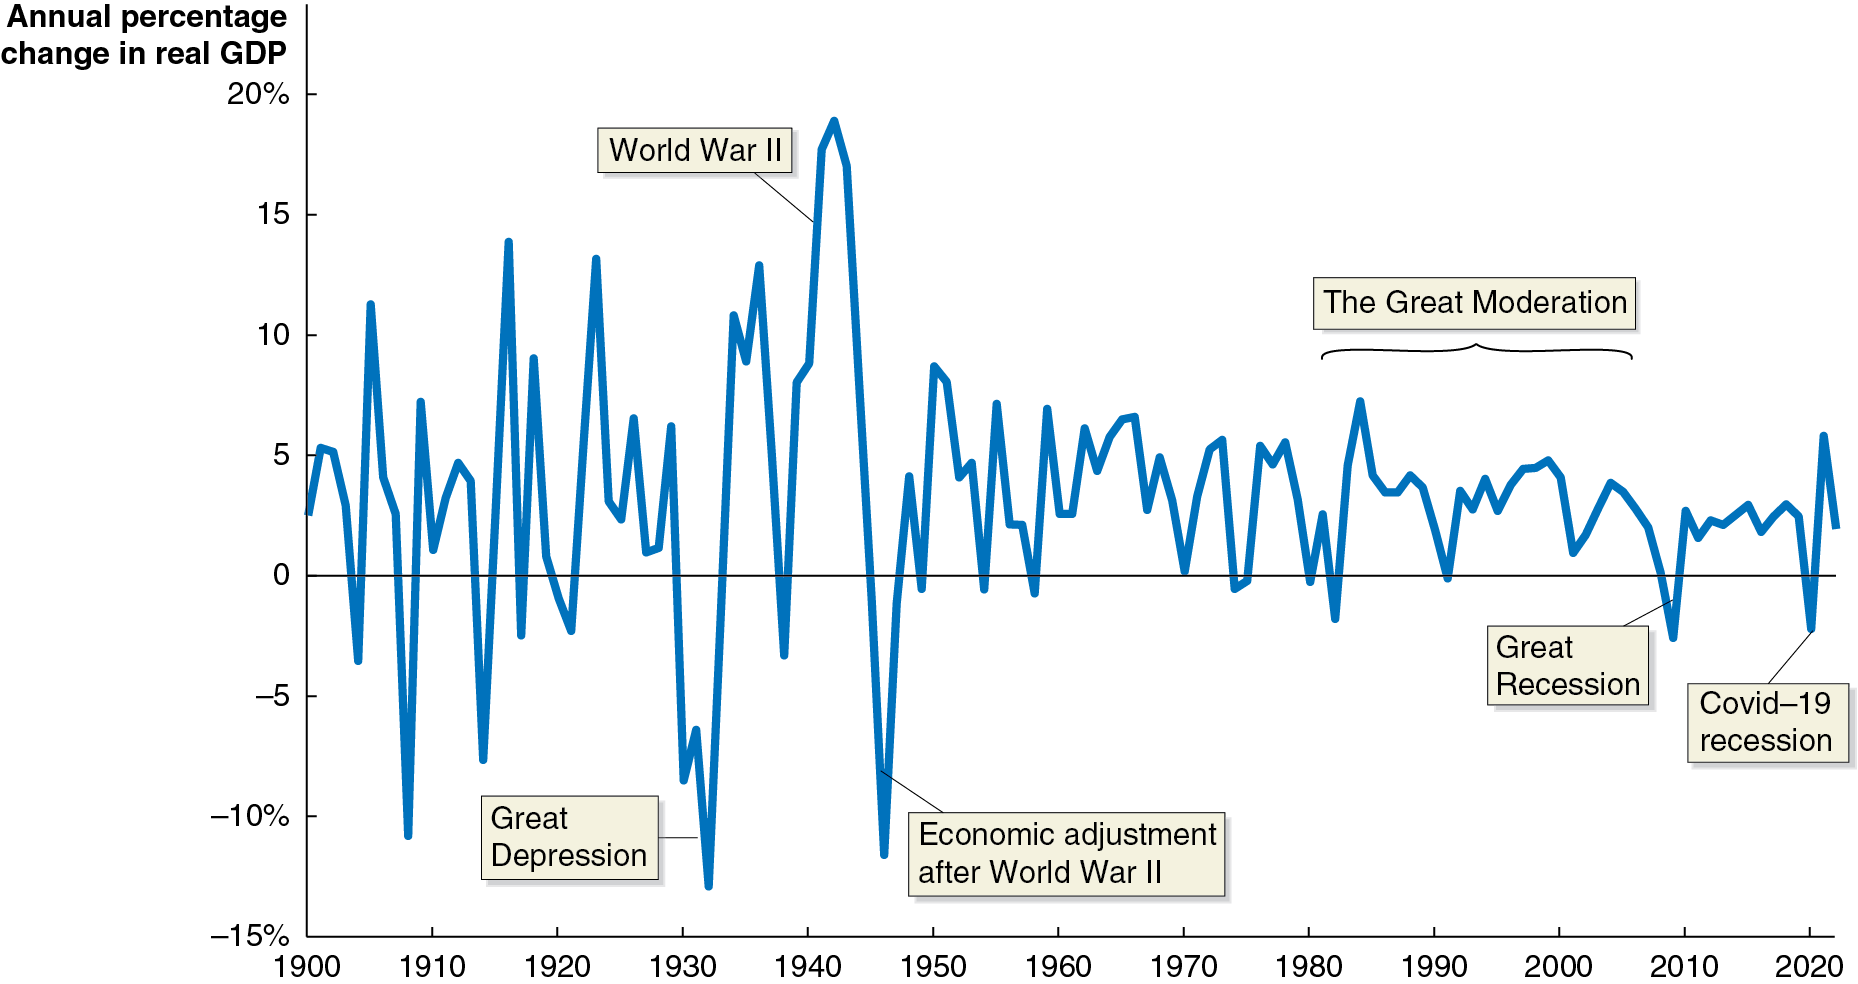
\includegraphics[width=\textwidth,height=0.99\textheight]{imgs3/img_slide44a.png}

Annual fluctuations in real GDP were typically greater before 1950 than
after 1950. + Business cycles have been particularly mild since the
mid-1980s, with some economists calling the ensuing period the Great
Moderation.
\end{frame}

\begin{frame}{Table 10.3 Until 2007, the Business Cycle Had Become
Milder}
\protect\hypertarget{table-10.3-until-2007-the-business-cycle-had-become-milder}{}
Table 10.3 Until 2007, the Business Cycle Had Become Milder

The length and severity of the recession of 2007--2009 made some
economists and policymakers wonder if we would return to the previous
pattern of long expansions and short, mild recessions. + But except for
the Covid-19 recession in 2020 and the subsequent strong recovery,
growth has been exceptionally stable.
\end{frame}

\begin{frame}{Can the U.S. Economy Return to Stability?}
\protect\hypertarget{can-the-u.s.-economy-return-to-stability}{}
Can the U.S. Economy Return to Stability?

Several factors help to explain the Great Moderation, and their
continuation suggests the U.S. economy will return to stability: + The
increasing importance of services + Manufacturing (especially of durable
goods) is more strongly affected by recessions. The economy is based
more on services now, decreasing the effect of the business cycle on
GDP.

The establishment of unemployment insurance + Before the 1930s,
unemployment insurance and other government transfer programs like
Social Security did not exist. These programs increase the ability of
consumers to purchase goods and services during recessions.
\end{frame}

\begin{frame}{Explaining the Great Moderation}
\protect\hypertarget{explaining-the-great-moderation}{}
Explaining the Great Moderation

Several factors help to explain the Great Moderation, and their
continuation suggests the U.S. economy will return to stability: +
Active federal government stabilization policies + Many, though not all,
economists believe that active government policies to lengthen
expansions and minimize the effects of recessions have had the desired
effect. The debate over the role of government in this way became
particularly intense during the recession of 2007--2009.

Increased stability of the financial system + The severity of the Great
Depression of the 1930s was in part caused by instability in the
financial system; similar instability exacerbated the recession of
2007--2009. Returning to macroeconomic stability will require a stable
financial system.
\end{frame}

\begin{frame}{Copyright}
\protect\hypertarget{copyright}{}
Copyright

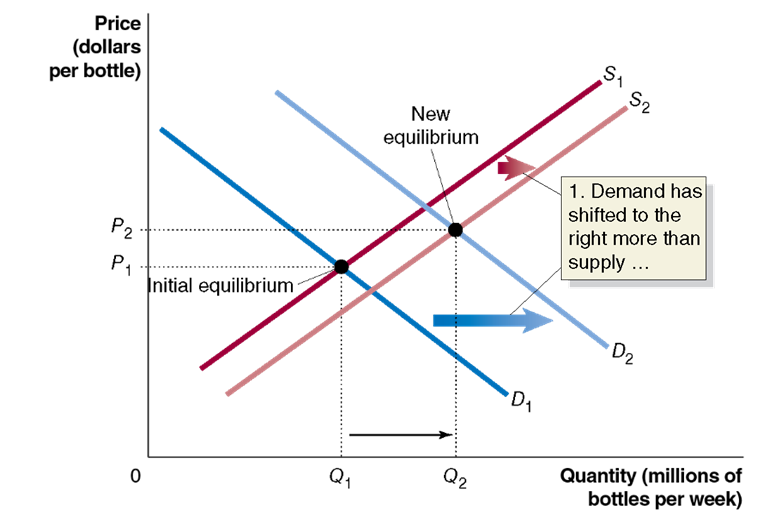
\includegraphics[width=\textwidth,height=0.99\textheight]{imgs3/img_slide48a.png}

This work is protected by United States copyright laws and is provided
solely for the use of instructors in teaching their courses and
assessing student learning. Dissemination or sale of any part of this
work (including on the World Wide Web) will destroy the integrity of the
work and is not permitted. The work and materials from it should never
be made available to students except by instructors using the
accompanying text in their classes. All recipients of this work are
expected to abide by these restrictions and to honor the intended
pedagogical purposes and the needs of other instructors who rely on
these materials.
\end{frame}

\end{document}
